\section{WiFi conditions}\label{sc:wifi}
In our test we used two different WiFi chanenls (4 and 11) and we found the best and the worst by using the WiFi Analyzer app from the Android app store\cite{Farproc@gmail.com2018}. As seen in figure \ref{fig:wifionthetestday}, channel 11 is used by Aarhus University WiFi but channel 4 looks rather free, so we picked these two as seen in table \ref{table:scenarios}.

\begin{figure}[h]
	\centering
	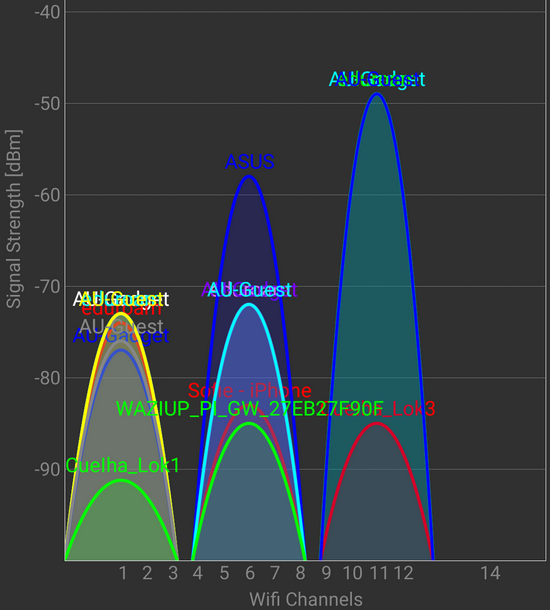
\includegraphics[width=0.6\linewidth]{testAndPerformance/wifi/wifiOnTheTestDay}
	\caption{WiFI on the test day. Channel 11 was busy and Channel 4 was a quiet channel}
	\label{fig:wifionthetestday}
\end{figure}
